\documentclass{article}


\usepackage{arxiv}

\usepackage[utf8]{inputenc} % allow utf-8 input
\usepackage[T1]{fontenc}    % use 8-bit T1 fonts
\usepackage{hyperref}       % hyperlinks
\usepackage{url}            % simple URL typesetting
\usepackage{booktabs}       % professional-quality tables
\usepackage{amsfonts}       % blackboard math symbols
\usepackage{nicefrac}       % compact symbols for 1/2, etc.
\usepackage{microtype}      % microtypography
\usepackage{lipsum}
\usepackage{multirow}
\usepackage{graphicx}

\title{Artist Identification	\\  A comparison between AlexNet, GoogLeNet and ResNeXt}


\author{
  Mattia Bottaro \\
  Dipartimento  di Matematica\\
  Università di Padova \\
  \texttt{mattia.bottaro@studenti.unipd.it} \\
  %% examples of more authors
   \And
  Mauro Carlin \\
Dipartimento  di Matematica\\
Università di Padova \\
\texttt{mauro.carlin@studenti.unipd.it} \\
  %% \AND
  %% Coauthor \\
  %% Affiliation \\
  %% Address \\
  %% \texttt{email} \\
  %% \And
  %% Coauthor \\
  %% Affiliation \\
  %% Address \\
  %% \texttt{email} \\
  %% \And
  %% Coauthor \\
  %% Affiliation \\
  %% Address \\
  %% \texttt{email} \\
}

\begin{document}
\maketitle

\begin{abstract}
	\textit{In this essay we present our work for the project of the Cognitive Services course.
	The problem we face is the artist identification task, that is being able to recognize the author of a painting, given an image of it.\\
	In order to resolve this task, we have exploited some differents Convolutional Neural Networks (CNNs) that come with \textit{Pytorch} library. Such networks have been trained in according to two distinct approaches: training them from scratch or exploiting pre-trained models using transfer learning technique. We used the \textit{Google Cloud Plataform} to train and evaluate our models.\\
	What we have achieved is a set of results which are in line with the  state-of-the-art, confirming that CNNs are suitable to solve this type of task.}
\end{abstract}


% keywords can be removed
\keywords{Convolutional Neural Networks \and Artist Identification \and CNNs \and ResNeXt \and GoogLeNet \and AlexNet \and Transfer Learning}


\section{Introduction}
\textbf{METTERE QUADRI ARTISTI (MAGARI STILI DIVERSI DELLO STESSO ARTISTA)}
Artist identification is a task regarding recognition of the painter who depicted a certain painting, given an image of it.\\
It's still nowadays a difficult problem to solve for the following reasons:
\begin{itemize}
	\item there are not many contributions yet and these rely on the latest models of deep learning (e.g. CNNs). 
	\item The available datasets are not as large as those used by models which solve more common tasks such as object detection or face recognition.
	\item An artist's style can change a lot through his works, or it could be influenced by other painters. For example, it is well known that Paul Cézanne and Camille Pissarro, who have spent a period of their lives together, have produced some works of similar style.
\end{itemize}
This type of task is still done by art experts and contributions to this type of problem can help and lead to the development of automatic fake artifact detection and automatic cataloguing of artworks.\\
We used three different CNNs: AlexNet (2012), GoogLeNet (2014) and ResNeXt (2016). For each of them, we have established two different ways of training: from scratch and with transfer learning  upon pre-trained version of such CNNs. Then we have observed and compared their performance. From our experiment we have obtained 83.768\% accuracy.\\


The rest of the essay is structured as follows: In section \ref{relwor} we discuss  similarities and differences between previous works and ours. In section \ref{dataset} we explain which dataset we have used, how it was formed and which preprocessing and data augmentation techniques we have exploited. In section\ref{method} we exhibit the CNNs' architectures and how we have trained them. In section \ref{experiments} we show some details regarding the \textit{GCloud Compute Engine}'s configuration, the metrics used to assess the goodness of the models and the detailed results of this experiment. Finally, in section \ref{conclusions} we draw some conclusion and we outline some possibile future works which rely on our result.


\section{Related Works}\label{relwor}

In this section we show some previous works related to ours. In addition to defining the references our experiment, the following should further convince the reader of present-day difficulty in achieving good precision in artist identification.\\
Recently CNNs have become widespread, this is due to the good performance and results obtained in this kind of task. In fact, we can distinguish the contributions to this task between those that come before the spreading of the CNNs, and thus do not use them, and those that instead benefit from it.\\
In our problem, the features that characterize an artist's style can be many and difficult to engineer, such as texture, shape, color, tone, variety, proportion, pattern and brush strokes.\\
Instead, it is well known that CNNs are able to learn those features that characterize an image, without having to identify and engineer a set of characterizing features.\\
In works prior to CNNs, some famous approaches of detection features are exploited, such as Scale Invariant Feature Transforms (SIFT) and Histograms of oriented gradients (HOG) (\cite{Saleh2015}, \cite{mensink2014}, \cite{lombardi05}, \cite{jou2011}). These works have in common the use of an SVM 1-vs-rest classifier, except \cite{jou2011} which uses both SVM 1-vs-rest and Naïve Bayes classifier.\\ However, \cite{lombardi05} and \cite{jou2011} face the problem of style recognition, which is different than artist identification.\\
In addition, some of these perform on small or not so heterogenous datasets, such as \cite{mensink2014} which uses the artwork of a single museum, or \cite{jou2011} which focuses on only 5 artists. Instead, in our work we focus on recognizing 23 different artists, and for each of them we take the same number of artifacts (\cite{ArtGANDataset}). \\

One of the results achieved in \cite{hong2017} shows the actual improvement of performance in the use of CNNs up to 13.6\% more than SIFT, HOG or similar.  This work aims to detect artwork that violates copyright terms in television programs, TV series, movies or similar scenarios. They use different techniques to distort the images on their dataset, which would not be suitable for our context. They experiment with three different CNNs inspired by AlexNet and VGG, then they trained them from scratch with a weights' initialization according to a Gaussian distribution. In our work, instead, we use pre-existing CNNs. \cite{hong2017} is one of the few works which does not use SVM as classifier, but 3 Fully Connected Layers, and the last of them is a Soft-Max layer.\\
Other works like \cite{Bar2014} and \cite{razavian2014} use a CNN to generate features, then use an SVM 1-vs-rest classifier on top of it.
\cite{ArtistIdCNN406} exploit one of the most recent CNNs: ResNet-18 (\cite{resnet}). It is an ancestor of ResNeXt (\cite{resneXt}), one of the CNNs used in our experiment. As in our work, also in \cite{ArtistIdCNN406} either training from scratch and training through transfer learning are studied.
\\

In the latest years, the number of CNNs for visual recognition task is growing, as well as their contributions in the field of computer vision. What is missing is a performance comparison between the latter models in the field of artist identification and, more generally, in art-recognition tasks. This comparison is the purpose of our work.

\section{Dataset}\label{dataset}


\subsection{Overview}\mbox{}\\
La prima cosa necessaria per allenare una cnn per questi task è un grande dataset di quadri di differenti artisti. Il dataset da noi utilizzato è preso da \cite{ArtGANDataset} che non è altro che un sottoinsieme del dataset Wikiart (cit link a wikiart). Si tratta di un dataset contenete circa 19k immagini di 23 artisti differenti , provenienti da epoche diverse fra loro, i quali hanno stili diversi fra loro, ma influenzati fra loro. Le immagini differiscono in dimensioni e forma.  Ci sono dei file .csv che contengono le label di ogni quadro suddividendo i quadri per  autore .Per avere un dataset bilanciato, abbiamo, per ogni artista, selezionato randomly 450 quadri.
L'organizzazione di \cite{ArtGANDataset} non presentava un test-set. Abbiamo quindi suddiviso i quadri in subset di train, validation e test con uno split 80-10-10, ottenengo quindi 360 quadri per il training, 45 per test e 45 per validation per ogni artista. In totale il numero complessivo di quadri è 10350.
Inoltre \cite{ArtGANDataset} presentava alcuni quadri in più subset, cosa da noi evitata in quanto ciò non porterebbe ad una corretta valutazione delle performance.
\subsection{Preprocessing and Data augmentation}\mbox{}\\
Per dare in input le immagini alle cnn è necessario che esse abbiano una certa forma e dimensione. Per ogni immagine prendiamo un crop di 224x224 e zero-centered (sottrarre la media) e normalization e utilizzando media e deviazioni standard per ogni channel (trattandosi di immagini RGB) red, green e blue. \\
Scrivere a cosa serve la data aug. Abbiamo utilizzato delle tecniche di data augmentation quali: per ogni immagine, prima di darla in input alla rete nella fase di training, abbiamo preso un crop 224x224 in una posizione casuale dell'immagine e flippato orizzontalmente con una prob del 50\%. Queste tecniche sono usate in task di visual recognition per aumentare il dataset e ridurre la possibilità di incorrere in overfitting.
Inoltre, per questo specifico task, ogni punto del quadro ha contenuto informativo sullo stile dell'autore.
\textbf{STUDIARSI COSA VUOL DIRE FARE NORMALIZATION (ZERO CENTER) E PERCHÈ È UTILE}.

\section{Method}\label{method}
abbiamo considerato tre reti cnn ossia, alexnet, googlenet e resnext.
Ad ogni rete abbiamo dato in input un'immagine RGB 3x224x224 e dato in output un valore di cofidenza per tutti e 23 gli artisti, prendendo il massimo come risultato della classificazione. 
Per ognuna delle reti abbiamo utilizzato un classifier softmax con cross entropy loss.
\begin{equation}
L_{i}=-\log \left(\frac{e^{f_{y_{i}}}}{\sum_{j} e^{f_{j}}}\right)
\end{equation}
Spiegare prendendo spunto.

Prima di tutto abbiamo allenanato le reti from scratch, in modo da cercare di imparare le features solamente per il compito di artisti identification.\\
Successivamente partendo dalle stesse architetture usando i pesi pretreinate sul ImageNet Dataset, per valutare se le features estratte per l'image recognition possono essere un buon punto di partenza per l'artist identification. Infatti ci aspettiamo che per determinati stili, come il Realism o reinassence, tali features possono essere utili, cosa non vera per cubismo, minimalismo, astrattismo.
\subsection{AlexNet}\mbox{}\\
AlexNet was the winning entry in ILSVRC 2012. It solves the problem of image classification where the input is an image of one of 1000 different classes (e.g. cats, dogs etc.) and the output is a vector of 1000 numbers, achieving a top-5 error of 15,8\%.
L'architettura è caratterizzata da 8 strati, 5 convolutional e 3 fully connected, con max pooling e ReLu come funzione di attivazione. RIFERIMENTO A IMMAGINE
Un'altra caratteristica di ALexnet è l'utilizzo della tecnica di dropout, introdotta nello stesso anno in \cite{dropout}, per ridurre l'overfitting. 
In dropout, a neuron is dropped from the network with a probability of 0.5. When a neuron is dropped, it does not contribute to either forward or backward propagation. 
As a result, the learnt weight parameters are more robust and do not get overfitted easily. \\

MOTIVAZIONE SCELTA


\subsection{GoogLeNet}\mbox{}\\
È stato il vincitore di ILSVRC 2014. It achieves 6.67\% top-5 error on ImageNet.
L'architettura è caratterizzata da 22 layer, con alcune novità per quanto riguarda gli strati fully connected, la gestione del problema del vanish del gradiente, e l'introduzione di un cossiddetto inception module.\\
Another interesting addition to the architecture is to change the second last fully-connected layer with an average pooling layer. This layer spatially averages the feature map, converting 7x7x1024 input to 1x1x1024, reducing the computation and the number of parameters, by a factor of 49. This average pooling layer is finally followed by a normal fully-connected layer with 1000 neurons (and 1024x1000 parameters), for the 1000 ImageNet classes.

During training, to address the vanishing gradient problem, special extra structures are added to the network (these are removed during testing). These are
auxiliary classifiers attached to intermediate layers. All the losses from each
classifier gets added up, taking contribution from the auxiliary classifier lower
than the main one, during training. The gradient from the main classifier which
would have otherwise become very small, and thus slowing training, by time it
reached the lower initial layers, receives gradient from the auxiliary classifiers
and thus the net gradient becomes big enough to allow training to progress.

\subsubsection{Inception Module}
Inception Modules are used in GoogLeNet to allow for more efficient computation through a dimensionality reduction with stacked 1x1 convolutions. The modules were designed to solve the problem of computational expense, as well as overfitting, among other issues. The solution, in short, is to take multiple kernel filter sizes within the CNN, and rather than stacking them sequentially, ordering them to operate on the same level. 

As a neural net deals with a vast array of images, with wide variation in the featured image content, also known as the salient parts, they need to be designed appropriately. The most simplified version of an inception module works by performing a convolution on an input with not one, but three different sizes of filters (1x1, 3x3, 5x5). Also, max pooling is performed. Then, the resulting outputs are concatenated and sent to the next layer.
A method to reduce the number of computation is dimensionality reduction. This involves convolutions with 1x1 filters before convolutions with bigger filters.

\subsection{ResNeXt}
ResNeXt was the first runner up in ILSVRC 2016, achieving 3.03\% top-5 error rate, superando la precisione umana.
Si tratta di una cnn residual, ossia presenta i cosiddetti residual block, (spiegazione residual).
The model name, ResNeXt, contains Next. It means the next dimension, on top of the ResNet, ossia la CNN vincitrice del  ILSVRC 2015. \\
This next dimension is called the “cardinality” dimension.
SPIEGARE NUOVO BLOCCO CON RIFERIMENTO A CARDINALITA

Noi abbiamo utilizzato 

\section{Experiments}\label{experiments}

\subsection{Setup}\mbox{}\\

Both the built models and the experiments have been implemented in Pytorch (\cite{pytorch}). The reason why we chose this library is because of the presence of models, pretrained and not, that we wanted to study.\\
The training of the models and the experiments were performed on a virtual machine (VM) hosted by \textit{Compute Engine}, one of the services provided by Google Cloud Platform (\cite{gcloud}). Its configuration, shown in table \ref{table:specVM}, is a pre-setting provided by the service itself and designed for deep learning applications  (\cite{vmconfig}). The dataset was stored in a \textit{Google Cloud Storage}'s Bucket, another service provided by Google Cloud Platform.

\begin{table}
	\centering
	\begin{tabular}{|l|l|} 
		\hline
		\textbf{Component} & \textbf{Specification}  \\ 
		\hline
		OS                 & Debian 9                \\
		vCPU               & 2                       \\
		RAM                & 13GB                    \\
		GPU                & 1X NVIDIA Tesla K80     \\
		Disk               & 100GB                   \\
		Disk Type          & SSD                     \\
		Availability Zone  & us-west1-b              \\
		\hline
	\end{tabular}
\\
\caption{VM specifications}
   	\label{table:specVM}
\end{table}

\subsection{Implementation Details}\label{ImplDet}

Per tutte le reti abbiamo testato le performance per diversi valori di LR, cioè da 10allameno2 a 10allameno5. Per ognuna di esse abbiamo riscontrato che lr=10allameno3 è il valore che permette di convergere più velocemente al miglior risultato e quindi tutti gli esperimenti riportati in questa sezione fanno riferimento a questo valore di lr. In tabella ?? riportiamo le performance di Resnext al variare di tale valore.

We chose the Adam's update rule because the experiments using SGD were worse. \textbf{Abbiamo impostato il }learning rate $= 10^{-3}$ mentre per gli altri papametri we used the default ones, i.e. $\beta_{1}  = 0.9$ and $\beta_{2} = 0.999$.  \textbf{MA COSA SONO beta1 e BETA2}\\

In transfer learning training, we set the number of epochs and the batch size to 15 and 32 respectively.  For each model chosen, pytorch makes available the final weights of these models trained on the ImageNet dataset (\cite{imagenet}), which makes transfer learning very easy to exploit.\\
\textbf{We first start training the network updating the weights only in the FC-layers, ma i risultati ottenuti non erano buoni}.\\
With the aim of achieving higher accuracy, \textbf{come sperimentato} in \cite{ArtistIdCNN406}, we have decided to allow the update of the weights in the whole network if, for 3 consecutive epochs, the validation set's accuracy does not improve by 3 percentage points. When this condition occurs, learning rate is decreased by a factor of 10. This strong decrease is motivated by the fundamental idea of the use of transfer learning: it is assumed that the pre-trained weights are already "close" or enough good to those we are looking for, so it is good to search for them with a relatively small step-size.
\\

In training from scratch, the number of epochs was set to 20, while the batch size remained 32.\\ 
Initialisation of the weights follows a uniform distribution in $[-x, x]$ where $x=1/\sqrt n$ and $n$ is the number of inputs to a given neuron (\textbf{STA COSA È DA VERIFICARE})\\
We have experimented what in pytorch is called \textit{scheduler}, i.e. every 7 epochs the learning rate is decreased by a factor of 10 . This strategy, however, has not led to improvements and in fact the results exposed have been obtained without the use of this technique.

\subsection{Evaluation metrics}
Per valutare le nostre reti abbiamo calcolato la top-1 accuracy, ossia quando un quadro viene classificato del pittore esatto, e la top-3 accuracy, ossia un quadro viene classificato correttamente se il suo autore e' compreso tra i 3 risultati con highest score generato dalla rete.

Infine i risulati ottenuti, oltre a confoirntarli tra di loro, li abbiamo conforntati con [mettere citazione], che e' il lavoro piu simile al nostro.

I riosultati piu' interessanti sono stati riportati sottoforma di grafico o tabella nella prossima sezione results.

\subsection{Results}\mbox{}\\

La tabella X contiene i risultati complessivi ottenuti per le varie reti, sia per quanto riguarda il training from scratch (left) che per l'allenamento with transfer learning (right), comprendendo anche il riferimento ai rusultati di \cite{ArtistIdCNN406}.\\
Il primo aspetto che possiamo notare, confrontando le nostre 3 reti, e' che AlexNet ottiene performance nettamente peggiori in tutti gli esperimenti, questo ci fa capire come effettivamente la complessita', profondita' crescente della rete permetta di raggiungere risultati migliori, cosa che ci si aspettava.
In particolare, nell'allenamento from scratch essa ottiene un 20\% in meno di accuracy, rispetto le altre reti, che diventa circa un 10\% di media nel transfer learning, dimostrando come il transfer learning sia un ottima tecnica per ottenere rislutati discereti anche con reti non troppo complesse (87\% di top-3 accuracy nel test set).

SCRATCH-LEARNING
Per tutte le reti possiamo notare come l'allenamento with tl ottiene risutalti circa 40\% migliori rispetto al from scratch. Questo ci fa capire come il pre-trained su imagenet, dataset molto piu ampio del nostro, sia un ottimo punto di partenza e che quindi i task di image classification e artist identification si assomiglino. RIGUARDARE \textit{a feature representation from ImageNet is a valuable starting point for artist identification. }

La nostra rete migliore risulta quindi essere Resnext with transfer learning, raggiungegngo un ottimo 80\% di top-1 accuraci e 93 nella top-3, meaning that it can narrow down the artist to three in the vast majority
of cases. 


CONFUSION MATRIX 
Figure 4 shows a confusion matrix. Each row represents the true artist and each column represents a predicted artist. Ideally, we want as many predictions as possible to be concentrated on the diagonal as this means that the network correctly predicted the true artist. The maximum possible value for a cell in the confusion matrix is 45, since there are 45 paintings per artist in the dataset.\\
In generale possiamo vedere come la maggior parte dei quadri venga classficata nel modo corretto, con i colori della diagonale rossi e gialli, ossia maggiore di 30 su 45. 

Nel dettaglio gli artisti che ottengono una precisione maggiore (44/45) sono Boudin, aivazovsky, kirchner. Ad esempio Ivan Aivazovsky produced many portraits and landscapes, over half of all of his paintings are realistic depictions of coastal scenes and seascapes. La caratteristica di dipengere scene o oggetti reali, rende la classificazione di questi quadri maggiormente simile all' iomage classification e dai risulati che abbiamo ottenuto notiamo che i pittori con quadri con queste caratteristiche ottengono una accuracy nella classficiazione migliore.

Negli aertisti che hanno ottenuto una accuracy piu' bassa abbiamo notato delle caratteristiche comuni. Alcuni di essi fanno parte di stili come il surrealismo, cubismo o espressionismo che li porta a reallizare quadri che non rappresentato la realta', quindi piu difficli da classificare; infatti pablo Picasso, il fondatore del cubismo, ottiene le performance peggiori (30/45). \\
Un altro motivo che porta alla miss-classfication e' la somiglianza dei quadri tra diversi artisti. L'esempio piu' evidente lo si ha in Ilya Repin, infatti la rete ha predetto Kustodiev come l'artista di 8 quadri di Repin. Questo non e' un fatto cosi sorprendente in quanto Ilya Repin e' stato l'insegnate di Boris Kustodiev, influenzato notevolmente il suo stile.
Un'ultima considerazione riguarda artisti che hanno prodotto quadri con stili molto diversi tra di loro, come possiamo vedere nella Figura X dove sono rappresentati due quadri di Van Gogh. Questo complica notevolmente la classificazione, portando in qualche caso a una accuracy non ottimale (Van Gogh 33/45)


ANDAMENTI ACCURACY

In figure \ref{fig:accscratch} vediamo l'andamento della top-1 acc sul training e validation set delle varie CNNs allenate from scratch. Ciò che si vede su tutte le reti è che le accuracy sul validation set e sul training set hanno andamenti simili, provando che i modelli non sono soggetti ad overfitting.\\
Alla luce di ciò, con un dataset più vasto e un maggior numero di epoche, si potrebbero ottenere performance ancora migliori.



In figure \ref{fig:acctransfer} vediamo invece l'andamento della stessa metrica sulle reti allenate con transfer learning.  
In tutte le reti, after few epochs, si nota un deciso incremento della pendenza. Questo corrisponde al momento in cui viene data la possibilità alla rete di aggiornarne non solo i pesi dei FC, ma anche di quelli di tutta la rete, come precedentemente esposto in \ref{ImplDet}. Da questo si intuisce che le reti pre-trained cercano di adattarsi all'artist identification.\\

Si nota inoltre che Googlenet e resnext, dopo circa 10 epoche, sono affette dall'overfitting. Infatti si vede una progressiva crescita nella differenza fra le due accuracy. Questo ci fa capire che per queste due reti poteva bastare un numero minore di epoche.  Comunque sia i risultati ottenuti sono migliori di quelli dei related works.


% Please add the following required packages to your document preamble:

\begin{table}[]
	\begin{tabular}{|c|c|c|c|c|}
		\hline
		\multicolumn{5}{|c|}{\textbf{Training from scratch}}                                                          \\ \hline
		\multirow{2}{*}{\textbf{Network}} & \multicolumn{2}{c|}{\textbf{Top-1}} & \multicolumn{2}{c|}{\textbf{Top-3}} \\ \cline{2-5} 
		& Train acc        & Test acc         & Train acc        & Test acc         \\ \hline
		AlexNet                           & 0.23103          & 0.27439          & 0.46159          & 0.51304          \\ \hline
		GoogLeNet                         & 0.42669          & 0.46956          & 0.68285          & 0.70628          \\ \hline
		ResNeXt-50                        & \textbf{0.50531} & \textbf{0.50048} & \textbf{0.74275} & \textbf{0.74782} \\ \hline
		ResNet-18 \cite{ArtistIdCNN406}                    & 0.516            & 0.511            & 0.737            & 0,710            \\ \hline
	\end{tabular}
	\begin{tabular}{|c|c|c|c|c|}
		\hline
		\multicolumn{5}{|c|}{\textbf{Training with transfer learning}}                                                           \\ \hline
		\multirow{2}{*}{\textbf{Network}} & \multicolumn{2}{c|}{\textbf{Top-1}}  & \multicolumn{2}{c|}{\textbf{Top-3}} \\ \cline{2-5} 
		& Train acc        & Test acc          & Train acc         & Test acc        \\ \hline
		AlexNet                           & 0.7134           & 0.68695           & 0.88925           & 0.87439         \\ \hline
		GoogLeNet                         & 0.87536          & 0.80579           & 0.96787           & 0.92492         \\ \hline
		ResNeXt-50                        & \textbf{0.91413} & \textbf{0.812560} & \textbf{0.98417}  & \textbf{0.9343} \\ \hline
		ResNet-18 \cite{ArtistIdCNN406}                    & 0.907            & 0.777             & 0.973             & 0.898           \\ \hline
	\end{tabular}
\end{table}



\begin{figure}[htp]
	
	\centering
	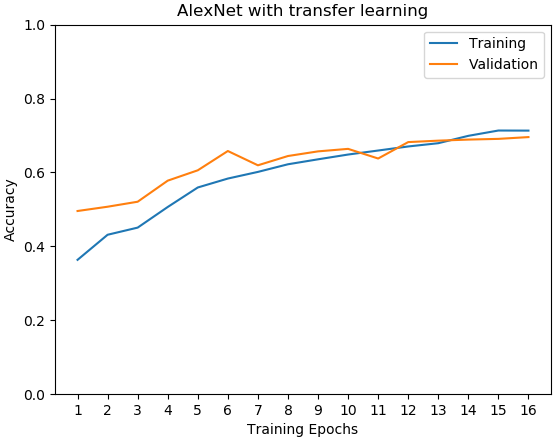
\includegraphics[width=.33\textwidth]{graphs/alex_training}\hfill
	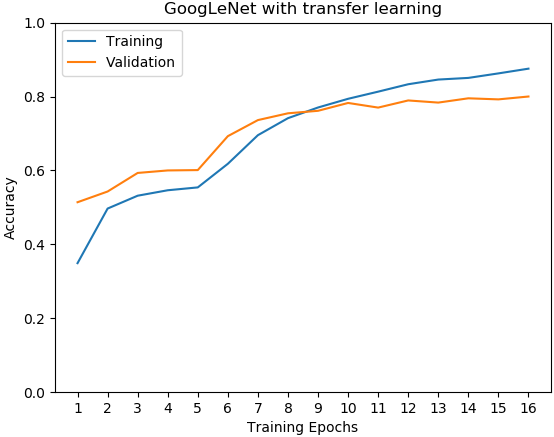
\includegraphics[width=.33\textwidth]{graphs/google_training}\hfill
	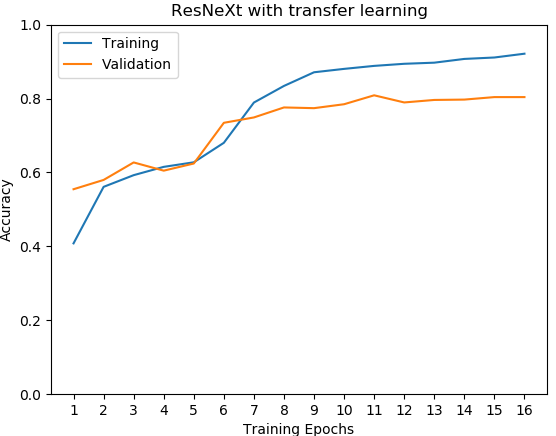
\includegraphics[width=.33\textwidth]{graphs/res_training}
	
	\caption{default}
	\label{fig:acctransfer}
	
\end{figure}

\begin{figure}[htp]
	
	\centering
	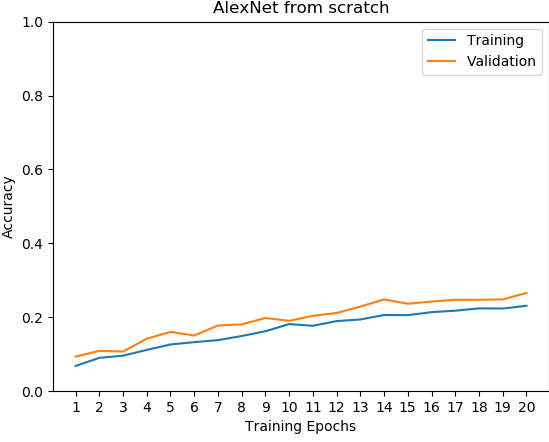
\includegraphics[width=.33\textwidth]{graphs/alex_scratch}\hfill
	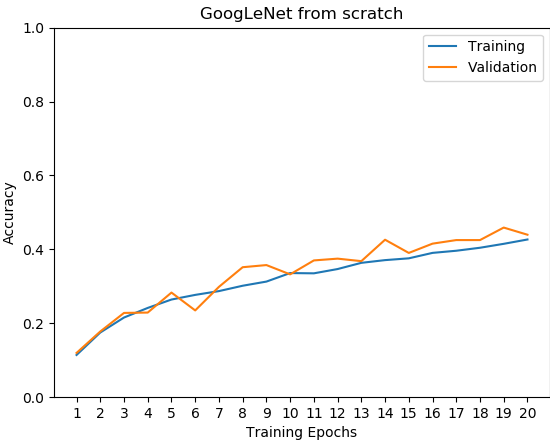
\includegraphics[width=.33\textwidth]{graphs/google_scratch}\hfill
	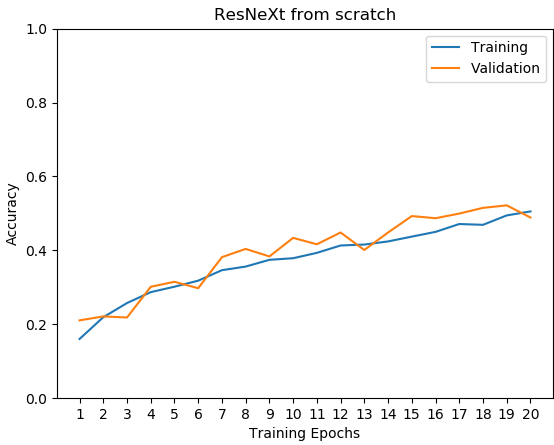
\includegraphics[width=.33\textwidth]{graphs/res_scratch}
	
	\caption{default}
	\label{fig:accscratch}
	
\end{figure}
\begin{figure}
	\centering
	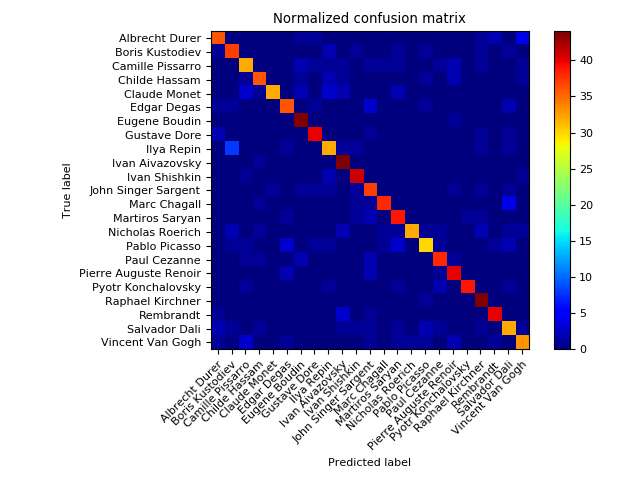
\includegraphics[width=0.8\linewidth]{graphs/confusion}
	\caption{Confusion matrix for top-1 classification on ResNeXt test set}
	\label{fig:confusion}
\end{figure}


\begin{figure}[htp]
	
	\centering
	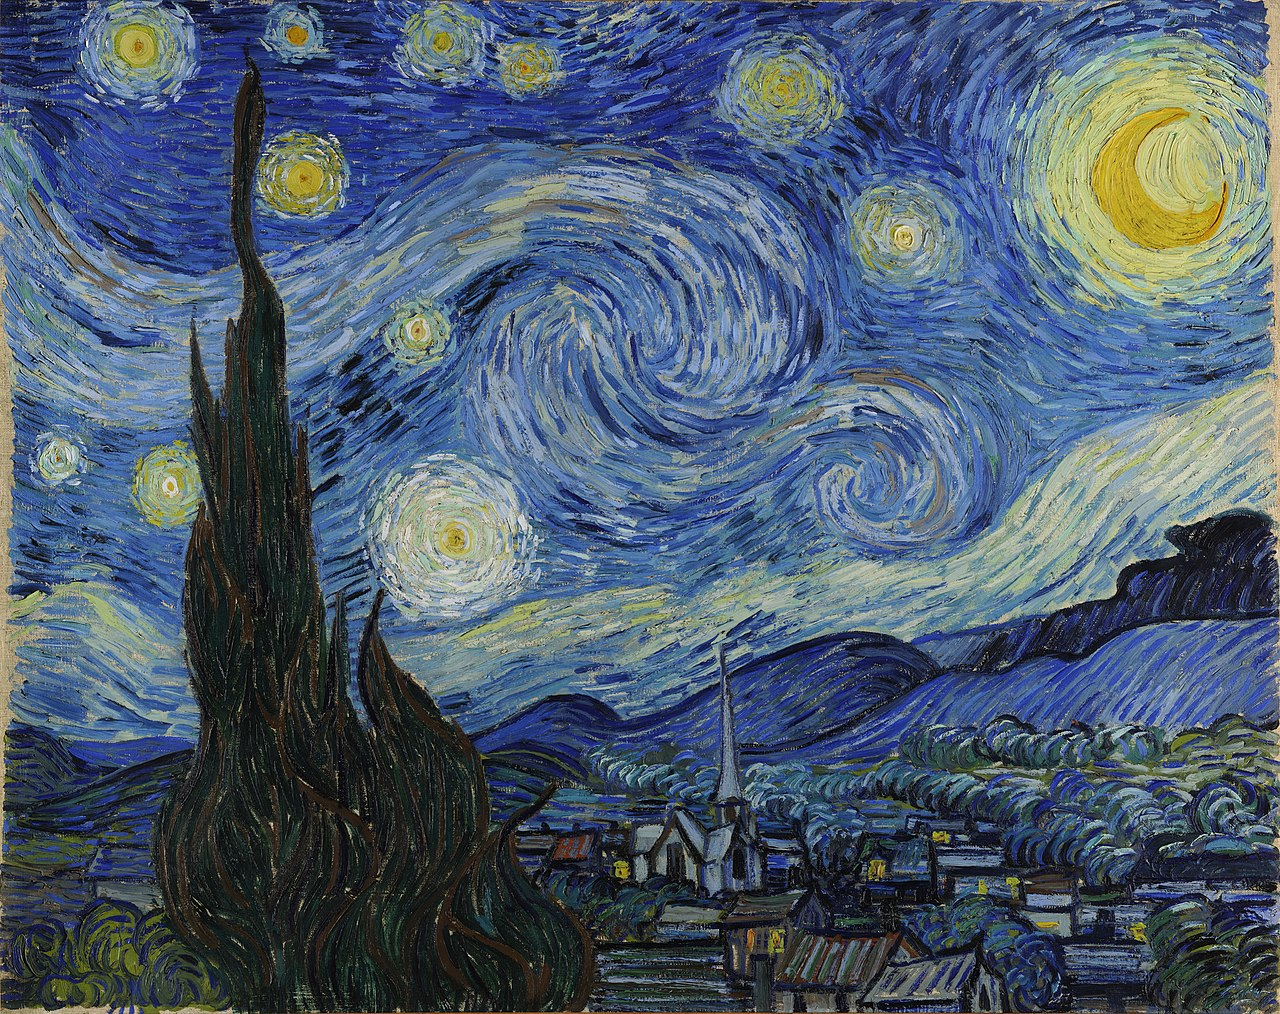
\includegraphics[width=.5\textwidth]{image/1280px-Van_Gogh_-_Starry_Night_-_Google_Art_Project}\hfill
	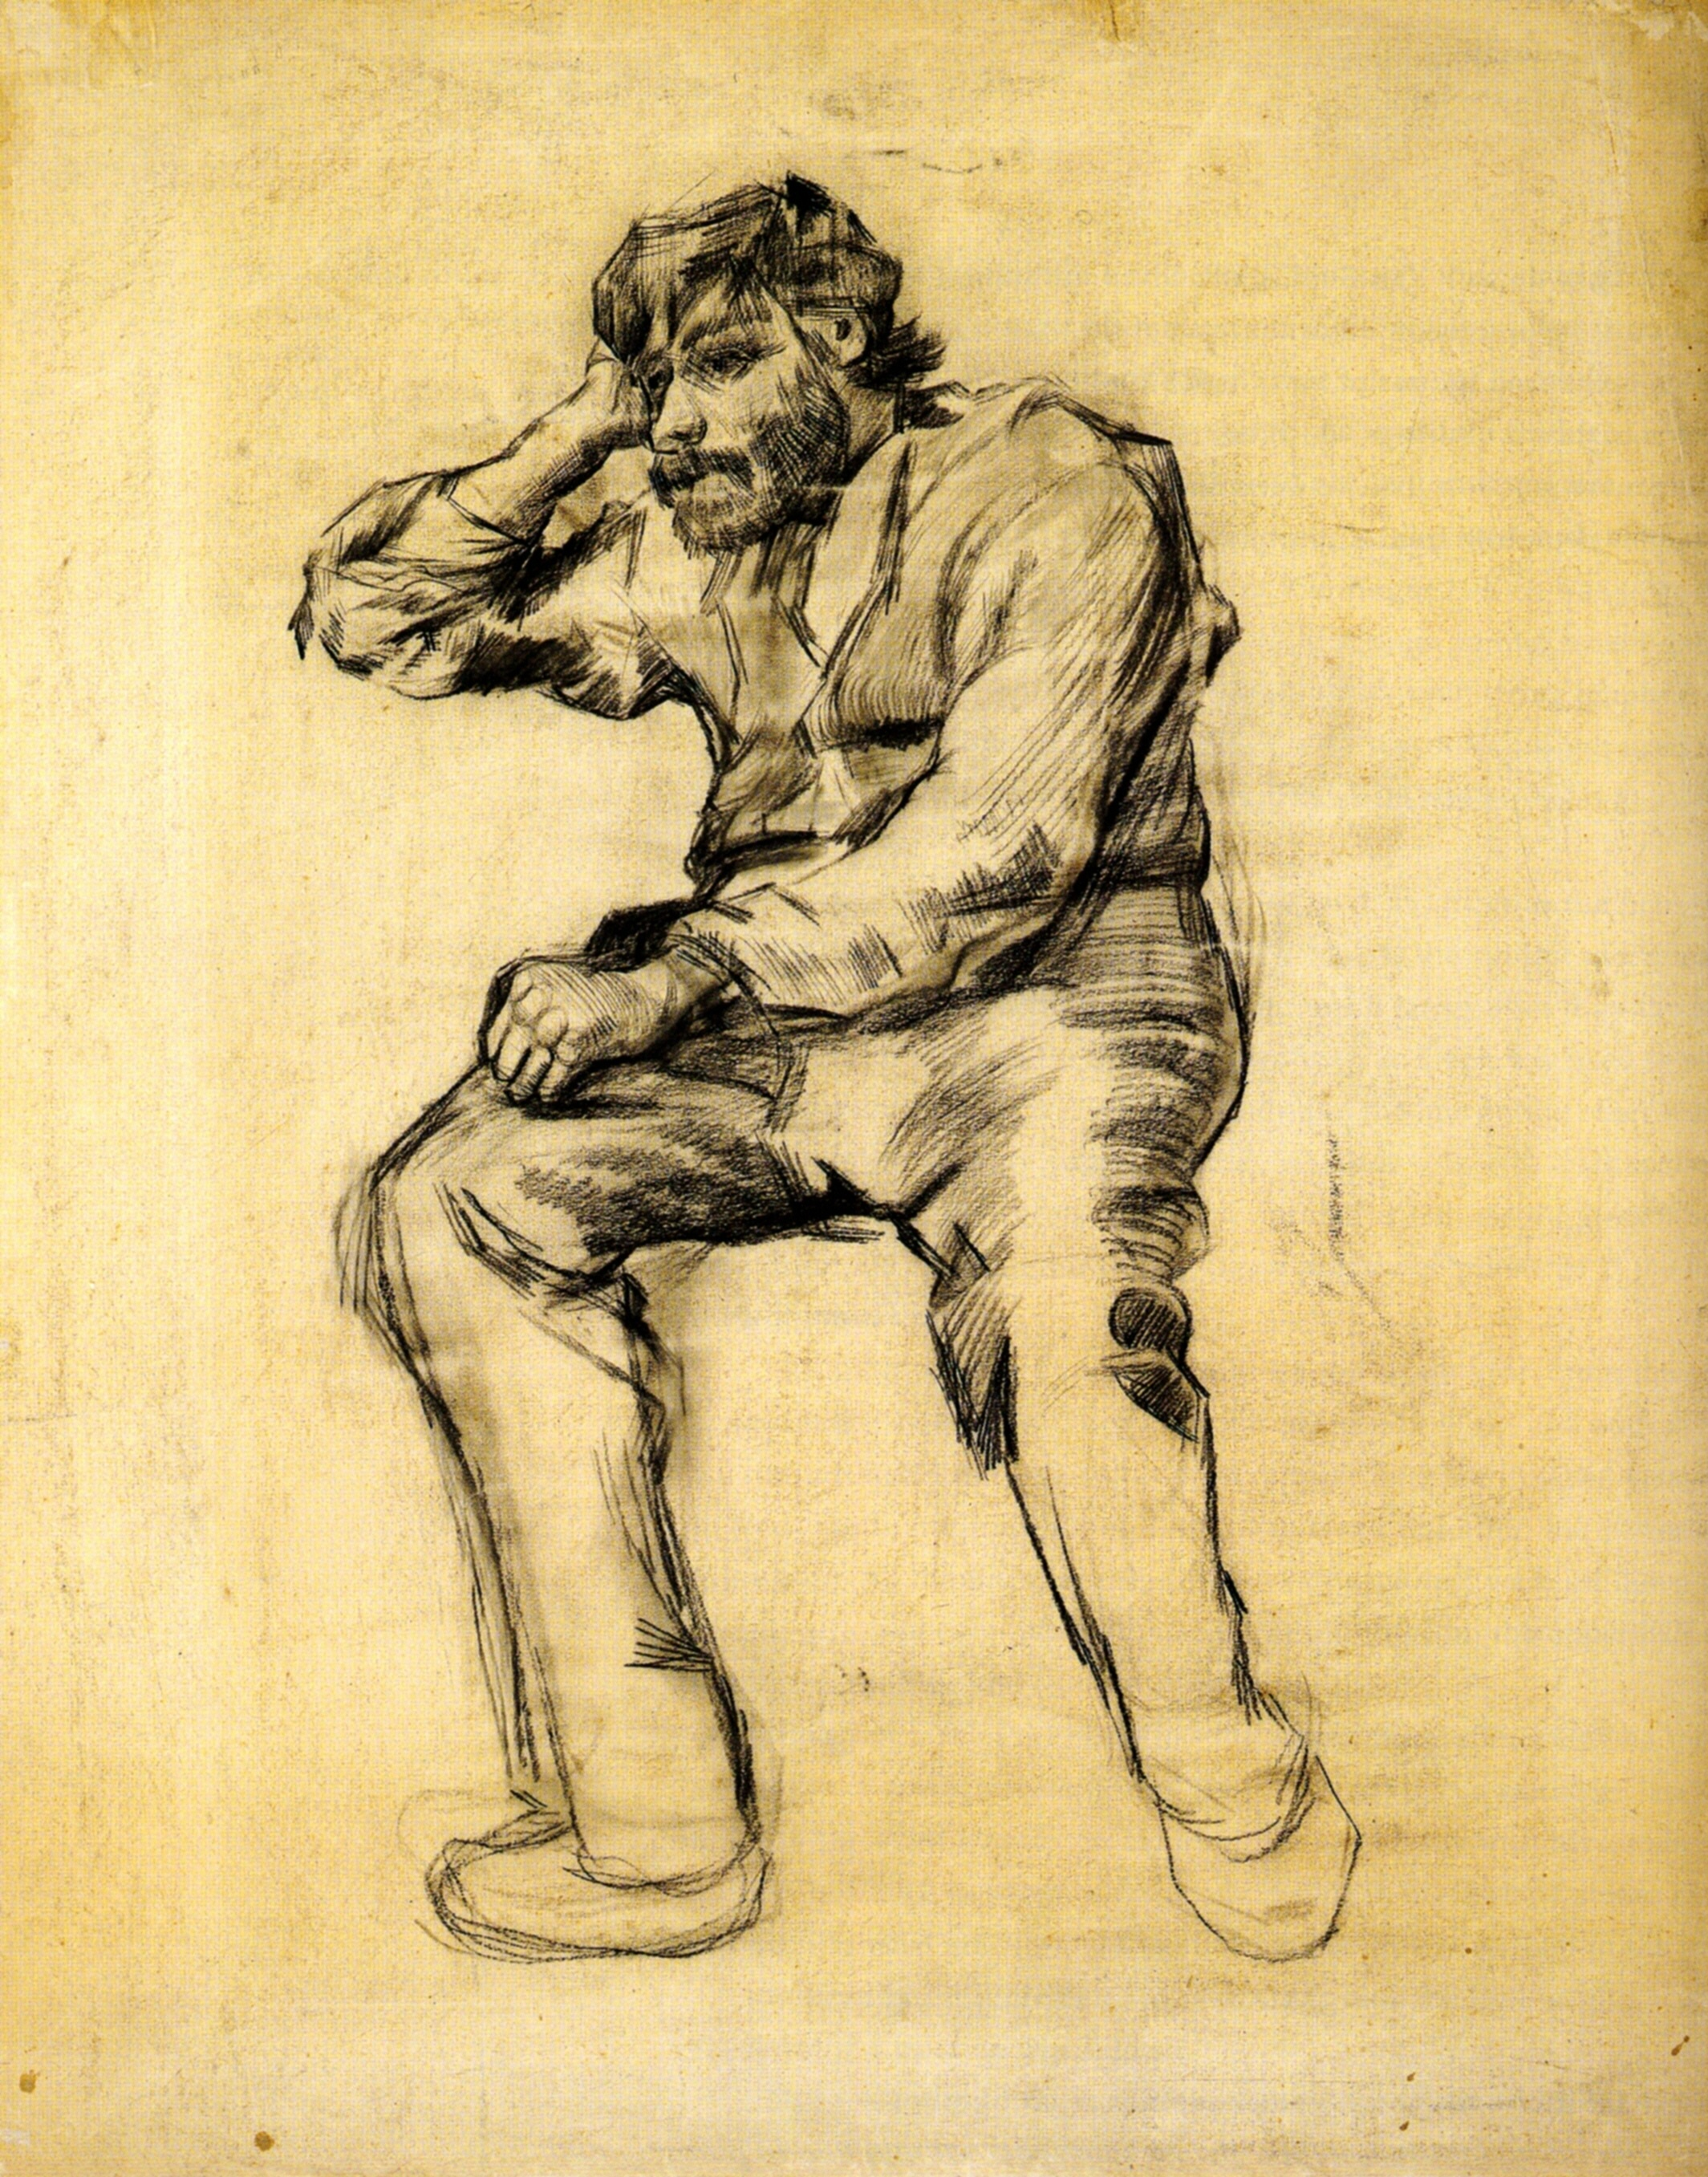
\includegraphics[height=.5\textwidth]{image/vincent-van-gogh_seated-man-with-a-beard-1886-1}
	
	\caption{default}
	\label{fig:vangogh}
	
\end{figure}

\section{Conclusions}\label{conclusions}

%%% Comment out this section when you \bibliography{references} is enabled.
\begin{thebibliography}{1}
	
	\bibitem{hong2017}
	Yiyu Hong, Jongweon Kim, \newblock  Art Painting Identification using Convolutional Neural Network, \newblock International Journal of Applied Engineering Research, \newblock 2017
	
	\bibitem{Saleh2015}
	B. Saleh and A. M. Elgammal.\newblock  Large-scale classification
	of fine-art paintings: Learning the right metric on the right
	feature. \newblock CoRR, abs/1505.00855, 2015.
	\bibitem{Bar2014}
	W. L. Bar Y., Levy N. Classification of artistic styles using binarized features derived from a deep neural network.
	ECCV 2014.
	
	\bibitem{mensink2014}
	T. Mensink and J. van Gemert. \newblock The rijksmuseum challenge:
	Museum-centered visual recognition. \newblock 2014
	
	
	\bibitem{ArtistIdCNN406}
	Nitin Viswanathan, Standford University,
	\newblock Artist Identification with Convolutional Neural Networks, \newblock 2017
	
	\bibitem{ArtGANDataset}
	Dataset:
	\url{https://github.com/cs-chan/ArtGAN/tree/master/WikiArt Dataset}
	
	\bibitem{Lij2012}
	E. H. J. Li, L. Yao and J. Z. Wang. \newblock Rhythmic brushstrokes
	distinguish van gogh from his contemporaries: Findings via
	automated brushstroke extractions. IEEE Trans. Pattern
	Anal. Mach. Intell, \newblock 2012.
		
	\bibitem{lombardi05}
	T. E. Lombardi. \newblock The classification of style in fine-art painting. ETD Collection for Pace University, \newblock 2005.
	
	\bibitem{jou2011}
	J. Jou and S. Agrawal. Artist identification for renaissance
	paintings, 2011.
	\bibitem{razavian2014}
	A. H. S. J. C. S. Sharif Razavian, A. Cnn features off-theshelf: An astounding baseline for recognition, 2014.
	
	\bibitem{resnet}
	Kaiming He, Xiangyu Zhang, Shaoqing Ren, Jian Sun. Microsoft Research. 
	Deep Residual Learning for Image Recognition. 2015
	
	\bibitem{resneXt}
	Saining Xie, Ross Girshick, Piotr Dollar, Zhuowen Tu, Kaiming He. UC San Diego - Facebook AI Research. Aggregated Residual Transformations for Deep Neural Networks, 2017.
	
	\bibitem{googlenet}
	Christian Szegedy, Wei Liu, Yangqing Jia, Pierre Sermanet, Scott Reed, Dragomir Anguelov, Dumitru Erhan, Vincent Vanhoucke, Andrew Rabinovich. Going Deeper with Convolutions. 2014
	
	\bibitem{alexnet}
	Alex Krizhevsky, Ilya Sutskever, Geoffrey E. Hinton. ImageNet Classification with Deep Convolutional
	Neural Networks. 2012
	
	\bibitem{dropout}
	G. E. Hinton, N. Srivastava, A. Krizhevsky, I. Sutskever and R. R. Salakhutdinov.
	Improving neural networks by preventing co-adaptation of feature detectors. 2012
	
	\bibitem{imagenet}
	ImageNet: \url{http://www.image-net.org/}
	
	\bibitem{pytorch}
	Pytorch: \url{https://pytorch.org/}
	
	\bibitem{vmconfig}
	Virtual Machine pre-settings: \url{https://console.cloud.google.com/marketplace/details/click-to-deploy-images/deeplearning}
	
	\bibitem{gcloud}
	Google Cloud Platform: \url{https://cloud.google.com/}
	
\end{thebibliography}


\end{document}

\end{document}